\documentclass[12pt]{reportj}
%Uncomment this if you want to use BibTeX
% RCS_ID: $Id: cos_isr_2018.tex,v 1.2 2018/02/27 18:02:38 penton Exp penton $
\usepackage{astron}
\usepackage{deluxetable}
\usepackage{times}
\usepackage{graphicx}
\DeclareGraphicsRule{.ps}{eps}{.ps}{}
\setlength{\headheight}{5mm}
\setlength{\headsep}{10mm}
\setlength{\footskip}{10mm}
\setlength{\textheight}{220mm}
\setlength{\textwidth}{170mm}
\setlength{\topmargin}{-8.0mm}
\setlength{\oddsidemargin}{+6.0mm}
\setlength{\evensidemargin}{+6.0mm}
\setlength{\parskip}{1mm}
\setlength{\parsep}{100mm}
\setlength{\parindent}{10mm}
\def\arcsec{\hbox{$^{\prime\prime}$}}
\def\degree{$^{\circ}$}
\usepackage{fancyheadings}
\pagestyle{fancy}
\newcommand*{\myfont}{\fontfamily{rm}\selectfont}
\def\numpos{{\bf NUM$\_$POS}\rm}
\def\acqimageno{{\myfont ACQ/IMAGE}\rm}
\def\acqimage{{\myfont ACQ/IMAGE}\rm~}
\def\acqimages{{\myfont ACQ/IMAGE{\rm s}}\rm~}
\def\acqsearch{{\myfont ACQ/SEARCH}\rm~}
\def\acqpeakd{{\myfont ACQ/PEAKD}\rm~}
\def\acqpeakxd{{\myfont ACQ/PEAKXD}\rm~}
\def\acqpeakds{{\myfont ACQ/PEAKD{\rm s}}\rm~}
\def\acqpeakxds{{\myfont ACQ/PEAKXD{\rm s}}\rm~}

%%%%%%%%%%%%%%%%
%For numbered sections use ssection/ssubsection/ssubsubsection. For sections without numbers user ssectionstar/ssubsectionstar/ssubsubsectionstar
%%%%%%%%%%%%%%%%
\def\ssection#1{\addtocounter{section}{1} \setcounter{subsection}{0} \S*{\hbox to \hsize{\large\bf \arabic{section}. #1\hfill }}}
\def\ssectionstar#1{\S*{\hbox to \hsize{\large\bf #1\hfill}}}
\def\ssubsection#1{\addtocounter{subsection}{1} \setcounter{subsubsection}{0} \subsection*{\hbox to \hsize{\normalsize\bfseries\itshape \arabic{section}.\arabic{subsection} #1\hfill}}}
\def\ssubsectionstar#1{\subsection*{\hbox to \hsize{\normalsize\bfseries\itshape #1\hfill}}}
\def\ssubsubsection#1{\addtocounter{subsubsection}{1} \subsection*{\hbox to \hsize{\normalsize\it \arabic{section}.\arabic{subsection}.\arabic{subsubsection} #1\hfill}}}
\def\ssubsubsectionstar#1{\subsection*{\hbox to \hsize{\normalsize\it #1\hfill}}}
%Set the footer on the first page
\lhead{}
\cfoot{\rm \footnotesize \hspace{-1.5cm}\it{
Operated by the Association of Universities for Research in Astronomy, Inc.,
for the National Aeronautics \newline and Space Administration.}\hspace{2.0 cm}}
\setlength{\headrulewidth}{0pt}
\setlength{\footrulewidth}{0pt}
\setlength{\textwidth}{147mm}

\begin{document}
\vspace{-2.4cm}
\noindent\includegraphics*[width=0.295\linewidth]{new_st_logo.eps}

\vspace{-0.4cm}

\begin{flushright}
% Put the instrument, year, and ISR number here (and also below)
{\bf Instrument Science Report COS2016-XX(v1)}

\vspace{1.1cm}

%Put ISR Title
{\bf\Huge Cycle 21-24 COS Target Acquisition Monitoring}

\rule{0.25\linewidth}{0.5pt}

\vspace{0.5cm}
%Put Authors
Steven V. Penton$^1$
\linebreak
\newline
%Put Author's affiliations
\footnotesize{$^1$ Space Telescope Science Institute, Baltimore, MD}
\vspace{0.5cm}

% Date here below
09-Feb-2018
\end{flushright}

\vspace{0.1cm}
%%%%%%%%
%Abstract
%%%%%%%%
\noindent\rule{\linewidth}{1.0pt}
\noindent{\bf A{\footnotesize BSTRACT}}

{\it \noindent
Beginning with HST Cycle~21, a series of annual HST programs were executed to verify that COS Target Acquisitions (TA) were performing
nominally.  This ISR documents these programs for HST Cycles 21-24. During this period, all FUV exposures were executed at Lifetime Position 3 (LP3),
and all NUV exposures were obtained at the nominal (LP1) position.
These programs were designed to monitor numerous aspects of both imaging and spectroscopic COS TAs, including
checking the TA subarrays, monitoring the required flashes of the internal PtNe lamps, and evaluating the accuracy of
numerous COS flight software (FSW) patchable constants required for TA.

There are three COS TA modes, FUV spectroscopic, NUV spectroscopic, and NUV imaging.
This project verified that all three modes were behaving nominally in Cycle 21-24, and determined that no SIAF or FSW parameter updates were required during this time.
There were, however, changed required for MIRRORB NUV \acqimages. These changes included a changing of the lamp current from LOW to MEDIUM, an adjustment of the LTACAL exposure time, and a modification of both the MIRRORB WCA and PSA/BOA TA subarrays. }

\vspace{-0.1cm}
\noindent\rule{\linewidth}{1.0pt}
%%%%%%%%
%Contents
%%%%%%%%
\vspace{-0.3cm}
\ssectionstar{Contents}
\vspace{-0.3cm}

%%%%%%%%%%%%%%%%%%%
%May need to compile twice for page references
%%%%%%%%%%%%%%%%%%%
\begin{itemize}
\item Introduction (page \pageref{sec:Introduction})
\item Program Descriptions \pageref{sec:programs}
\item SIAF Verification (page \pageref{sec:siaf})
\item \acqimage Performance (page \pageref{sec:acqimage})
\item ACQ/PEAKXD Performance (page \pageref{sec:acqpeakxd})
\item TA Subarray Performance (page \pageref{sec:subarray})
\item Conclusion (page \pageref{sec:theend})
\end{itemize}
%%%%%%%%
%Body
%%%%%%%%
\clearpage
\ssection{Introduction}\label{sec:Introduction}

The basic results of the programs reviewed here were previously reported in the following COS ISRs:
\begin{itemize}
\item{COS ISR 2016-09 (Cycle 21 COS Target Acquisition Monitor Summary)}
\item{COS ISR 2017-09 (Cycle 22 COS Target Acquisition Monitor Summary)}
\item{COS ISR 2018-09 (Cycle 23 COS Target Acquisition Monitor Summary)}
\item{COS ISR 2018-09 (Cycle 24 COS Target Acquisition Monitor Summary)}
\end{itemize}
This ISR provides the full details of the following HST+COS Programs:
\begin{itemize}
\item{HST Program 13526 (COS Imaging TA and Spectroscopic WCA-PSA/BOA offset verifications, Cycle 21)}
\item{HST Program 13972 (COS Imaging TA and Spectroscopic WCA-PSA/BOA offset verifications, Cycle 22)}
\item{HST Program 14440 (COS Imaging TA and Spectroscopic WCA-PSA/BOA offset verifications, Cycle 23)}
\item{HST Program 14857 (COS Imaging TA and Spectroscopic WCA-PSA/BOA offset verifications, Cycle 24)}
\end{itemize}

There are three modes of COS Target Acquisition (TA); NUV imaging, NUV spectroscopic, and NUV imaging.
There are four COS TA (ACQ/) procedures; \acqimageno, PEAKD, PEAKXD, and SEARCH. The ACQ/PEAKD and SEARCH
step the telescope through dwell patterns on the sky. As long as the target light falls correctly within
the TA detector sub-arrays, ACQ/PEAKD and SEARCH will continue to nominally assist in TA (barring any
unforeseen anomalies). The \acqimage and PEAKXD procedures rely on the sub-arrays and patchable constants
in the COS flight software (FSW) which assist in target centering. In both \acqimage and PEAKXD, the internal
wavelength calibration lamp is flashed to locate the center of the wavelength calibration aperture (WCA). From this location, the center of the
science aperture (SA) in use can be predicted by applying the FSW constant that give the SA offset compared to the WCA center. For \acqimageno,
the offset is in both detector X (along-dispersion, AD) and Y (cross-dispersion, XD). For ACQ/PEAKXD, which
uses dispersed light, this offset is only in the Y (XD) direction. HST program 13972 also verifies that the TA subarrays
are proper and re-measures the actively used WCA-to-SA offsets to monitor the performance of COS TAs.

\acqimage has four combinations of two SAs, the Primary Science Aperture (PSA) and the Bright
Object Aperture (BOA), and two mirror modes, MIRRORA and MIRRORB. Each combination is commonly used, and has a slightly different
WCA-to-SA offset in both X (AD) and Y(XD), which must be verified. Each COS grating has a different WCA-to-SA XD offset.
BOA spectroscopic TAs are not supported for COS, so 13972 only verifies the WCA-to-PSA offsets that are used in ACQ/PEAKXD.
Each COS grating has a different offset, as do each of the FUV lifetime positions (LP). This program only verifies the NUV LP1
and FUV LP3\footnote{The COS FUV channel was moved to LP3 on February 15, 2015.} position offsets.

The centering requirements are based upon the wavelength accuracy requirements in the AD, and for flux and resolution optimization
in the XD. The strictest NUV requirements are [AD,XD] = [0.041, 0.3]\arcsec, while for the FUV they are [AD,XD] = [0.106, 0.3]\arcsec. The XD
requirement is that all TAs center to within $\pm$ 0.3 \arcsec\ with a 1$\sigma$ goal of $\pm$ 0.1\arcsec.

In \S~\ref{sec:acqimage} we will discuss the verification of the FSW parameters associated with COS \acqimages.
Some data from visit 'A2' of program 14035 will be used to assist in this verification. This data will be used to verify
the COS NUV SIAF (Science Instrument Aperture File) entries. In ~\S~\ref{sec:peakxd},
we will discuss the verification of the FSW parameters associated with COS ACQ/PEAKXDs, and the verification of the
COS FUV SIAF entries.

All 13972 data were taken on October 6, 2015, while the data in 14035 used by this program (Visit A2) were taken on October 2, 2015.
These data were intentionally taken contemporaneously to avoid any long-term detector or spacecraft effects from affecting our results.\\

%!!!!!!!!!!!!!!!!!!!!!!!!!!!!!!!!!!!!!!!!!!!!!!!!!!!!!!!!!!!!!!!!!!!!!!!!!!!!!!!!!!!!!!!!!!!!!!!!!!!!!!!!!!!!!!!!!!!!!!!!!!!!!!!!!!!!!!!!!!!!!!!!!!!!!!!!!!!!!!!!!!!!!!!!!!!!!!!!!!!!!!!!!!!!!!!!!!!!!!!!!!!!!!!!!!!!!!!!!!!!!!!!!!!!!!!!!!!!!!!!
%THIS SECTION NEEDS TO GO AFTER THE END OF THE FIRST PAGE AND BEFORE THE END OF THE SECOND PAGE
%Fill in Instrument, Year, and ISR Number and delete "newpage" immediately after this message
%!!!!!!!!!!!!!!!!!!!!!!!!!!!!!!!!!!!!!!!!!!!!!!!!!!!!!!!!!!!!!!!!!!!!!!!!!!!!!!!!!!!!!!!!!!!!!!!!!!!!!!!!!!!!!!!!!!!!!!!!!!!!!!!!!!!!!!!!!!!!!!!!!!!!!!!!!!!!!!!!!!!!!!!!!!!!!!!!!!!!!!!!!!!!!!!!!!!!!!!!!!!!!!!!!!!!!!!!!!!!!!!!!!!!!!!!!!!!!!
\newpage

\lhead{}
\rhead{}
\cfoot{\rm {\hspace{-1.9cm} Instrument Science Report COS 2016-09(v1) Page \thepage}}

\clearpage
\ssection{Program Descriptions \label{sec:programs} }

In addition to 13972, COS exposures obtained in HST program 14035 (HST Cycle 22 Focal Plane Calibration (SI-FGS Alignment)) were used in this analysis.
This program builds upon the monitoring and calibration of the FGS-to-SI alignment program (14452 - HST Cycle 23- Focal Plane Calibration (SI-FGS Alignment)).  HST 14452 performs back-to-back PSA/MIRRORA and PSA/MIRRORB \acqimages, from which all the results herein are bootstrapped.

From Cycles 17-23, an FGS-to-SI program was repeated twice a year. These programs contained COS exposures designed to assist in the monitoring of the COS NUV alignent to HST.
These programs used the same two stars with COS in visits spaced six months apart. Both visits observed the astrometric open cluster M35, at orientations that were 180\degree apart.
The two stars observed were 206W3 (in the Fall) and 427W3 (in the Spring). Due to time constraints, the exact content of the COS visits in these programs varied from year to year.

However, the COS portion of each program begins with a PSA+MIRRORA \acqimage on a target should be approximately centered due to observations with other instruments earlier in the Visit.
Post-observation telemetry data, an the results of the \acqimage, are used to refine this assumption.
This process verifies the COS NUV PSA aperture position\footnote{Specifically, the \textit{LFPSAA} entry.} in the SIAF to about 0.5 pixels or (~0.012\arcsec).

After this PSA+MIRRORA \acqimageno, a PSA+MIRRORB \acqimage is then performed.
This exposure bootstraps the PSA+MIRRORB centering to the PSA+MIRRORA SIAF verification.
This allows us to monitor the properties of the PSA+MIRRORB image in a controlled way on a centered target.
No spectra are taken in 14452 due to time constraints, but we are currently planning on adding in PSA/MIRRORA and PSA/MIRRORB lamp images.

The historical list of FCS-to-SI proposals, cycles (C), and content were:
\begin{itemize}
	\item{11878 (C17)}{Two sets of PSA/MIRRORA + PSA/MIRRORB \acqimages, Target+Lamp Time-Tag images, \& G230L Spectra}
	\item{12399 (C18)}{Two sets of PSA/MIRRORA + PSA/MIRRORB \acqimages, One set of Target+Lamp Time-Tag images (427W3), one G230L Spectrum (427W3)}
	\item{12781 (C19)}{Two sets of PSA/MIRRORA + PSA/MIRRORB \acqimages}
	\item{13171 (C20)}{Two sets of PSA/MIRRORA + PSA/MIRRORB \acqimages}
	\item{13616 (C21)}{Two sets of PSA/MIRRORA + PSA/MIRRORB \acqimages}
	\item{14035 (C22)}{Two sets of PSA/MIRRORA + PSA/MIRRORB \acqimages}
	\item{14452 (C23)}{Two sets of PSA/MIRRORA + PSA/MIRRORB \acqimages, but with Lamp-Only Time-Tag images after each \acqimage}
\end{itemize}

This verifies the COS NUV PSA aperture position in the SIAF. After this PSA+MIRRORA \acqimageno, a PSA+MIRRORB \acqimage is then performed.
This exposure bootstraps the PSA+MIRRORB centering to the PSA+MIRRORA SIAF verification.
This allows us to monitor the properties of the PSA+MIRRORB image in a controlled way on a centered target.
No spectra are taken in 14452 due to time constraints, but we are currently planning on adding in PSA/MIRRORA and PSA/MIRRORB lamp images.

Visits 01 and 02 of this program extend the COS SIAF/FGS-to-SI verification of Visit 02 of 14452 to the other two \acqimage combinations (BOA+MIRRORA and BOA+MIRRORB) by bootstraping from the PSA+MIRRORB verification to co-align all the COS TA imaging modes.
The details of the observations are given is the observing section.

Visit 01 of this program bootstraps off Visit 02 of 14452  to co-align the PSA+MIRRORB \acqimage mode to the BOA+MIRRORA.
We prefer that Visit 01 of this program executes within 45 days of Visit 02 of 14452, to ensure that no long term instrument or telescope focus changes impact our results.

Visit 02 of this program follows the style of Visit 01,  and bootstraps from the BOA+MIRRORA mode to the BOA+MIRRORB TA imaging mode.
Visit 02 should also occur within 45 days of visit 02 of 14452 and within 45 days of Visit 01 of this program.

Visit 3 of this program is an on-hold, contingency visit that would be used to replace the 14452 Visit 02 in case this program is, for whatever reason, not executed as planned.
In this case the 1st \acqimage is PSA/MIRRORA and the 2nd \acqimage is PSA/MIRRORB.
This visit also takes several lamp images to measure the WCA-to-PSA imaging offset FSW patchable constants.

In all visits, lamp+target images are taken before and after the TA imaging mode that is being co-aligned (the second \acqimage of the program.)

All visits in this program are single orbit visits, this program is very similar to the C22 version (13972).
Due to the change in OSM2 Home position, some NUV spectra have been re-ordered for efficiency AND some NUV cenwaves were changed to those that are known to have good stripe B WCA spectra.
\clearpage
\ssection{SIAF \label{sec:siaf} }

\ssection{Verifying the \acqimage WCA-to-SA Offsets.\label{sec:acqimage} }
\vspace{-0.3cm}

In the servicing mision orbital verification (SMOV) phase, a series of programs in NUV imaging mode
carefully determined the two-dimensional offset from the WCA to the center of the PSA when observed with MIRRORA.
These X and Y offsets were loaded in the FSW parameters {\it pcta\_XImCalTargetOffset} and {\it pcta\_YImCalTargetOffset}.
A target was then centered using a PSA+MIRRORA \acqimageno, then a target image was taken along with a MIRRORB image
of the WCA image. These images were used to determine the X and Y offsets of the image target and WCA centroids.
These values were uploaded in the FSW paramaters. This bootstrapping procedure was repeated with the BOA+MIRRORA
and BOA+MIRRORB \acqimage modes until all four \acqimage modes were co-aligned.

In this program (13972) we use this bootstrapping strategy to test the co-alignment of all four \acqimage modes.\footnote{On November 6, 2014,
the MIRRORB \acqimage wavelength calibration lamp exposure was changed from a 30 second exposure
at LOW current (3mA) to a 12 second exposure at MEDIUM current. At this point the {\it pcta\_XImCalTargetOffset} and {\it pcta\_YImCalTargetOffset}
FSW parameters were also updated to reflect a small change in the WCA-to-SA imaging MIRRORB offsets. This program is the first
to monitor the updated offsets.}
To accomplish this in only two orbits, this project leverages observations taken in FGS-to-SI alignment verification
program (14035).
\clearpage
The FGS-to-SI program (14035) performs a PSA/MIRRORA \acqimage on a target that should be centered in the aperture.
The PSA+MIRRORA \acqimage in Visit 'A2' of 14035 can be used to verify the COS NUV PSA aperture position in the SIAF.
This exposure shows that the COS NUV PSA SIAF entry combined with the PSA+MIRRORA WCA-to-PSA offsets are
accurate to within [AD,XD] = [-0.020,0.105]\arcsec\ (this is the distance that the \acqimage slewed to center the target).
The COS aperture is only repeatable in the XD direction to $\pm$ one motor step (0.05\arcsec). In addition, the WCA location
cannot be measured to better than 1/2 pixel as the pixel used to determine the median location in an integer.
On the NUV detector, 1 pixel is $\sim$ 0.023\arcsec. Based upon this information, the COS NUV PSA definition
in the SIAF file appears to meet our accuracy requirements for Cycle 22.

After the 14035 Visit 'A2' PSA+MIRRORA \acqimageno, a PSA+MIRRORB \acqimage is performed.
This exposure bootstraps the PSA+MIRRORB centering to the PSA+MIRRORA + SIAF verification.
This allows us to monitor the properties of the PSA+MIRRORB image in a controlled way on a centered target. No spectra or images are taken in 14035 due to time constraints.
Visits 01 \& 02 of 13972 extend the COS SIAF/FGS-to-SI verification of Visit 02 of 14035 to the other two \acqimage combinations (BOA+MIRRORA \& BOA+MIRRORB) by bootstraping from the PSA+MIRRORB verification to co-align all the COS TA imaging modes. The details of the observations are given is the observing section.
Visit 01 of 13972 bootstraps off Visit 02 of 14035 to co-align the PSA+MIRRORB \acqimage mode to the BOA+MIRRORA. Visit 01 of 13972 executed within 45 days of Visit 02 of 14035, to ensure that no long term instrument or telescope focus changes impact our results.
Visit 02 of 13972 follows the style of Visit 01, and bootstraps from the BOA+MIRRORA mode to the BOA+MIRRORB TA imaging mode. Visit 02 should also occur within 45 days of visit 02 of 14035 and within 45 days of Visit 01 of 13972.

The results of 13972 \& 14035 show that, for \acqimages :
\footnotesize
\begin{itemize}
\item PSA+MIRRORA is aligned with PSA+MIRRORB to [AD, XD] $\le$ [0.022, 0.007] \arcsec\ (14035, Visit 'A2')
\item PSA+MIRRORB is aligned with BOA+MIRRORA to [AD, XD] $\le$ [0.023, 0.100] \arcsec\ (13972, Visit '01')
\item BOA+MIRRORA is aligned with BOA+MIRRORB to [AD, XD] $\le$ [0.022, 0.024] \arcsec\ (13972, Visit '02')
\end{itemize}
\normalsize

These results can be combined to show the measured offsets of PSA+MIRRORB, BOA+MIRRORA, \& BOA+MIRRORB when compared
to the initial PSA+MIRRORA \acqimage of Visit 'A2' of 14035. These results are shown in Table~\ref{table:ai}.
Combined offsets from PSA+MIRRORA are provided in both NUV pixels (p) and in arcseconds (\arcsec).

\begin{deluxetable}{|r|r|r|r|r|r|}
\tabcolsep 10pt
\tabletypesize{\footnotesize}
\tablecolumns{6}
\tablewidth{0 pt}
\tablecaption{\acqimage WCA-to-SA offsets from PSA+MIRRORA\label{table:ai}}
\tablehead{\colhead{Aperture}&\colhead{MIRROR}&AD Offset & XD Offset & AD Offset& XD Offset\\
&&(\arcsec) & (\arcsec) & (p) & (p)
}
\startdata
\hline
PSA & B & 0.021 &-0.049 & 0.298 & 0.893\\
BOA & A & 0.010	& 0.060 & 0.425 & 2.550\\
BOA & B & 0.036	& 0.070 &1.530 & 2.975 \\
\hline
\enddata

\end{deluxetable}
\clearpage
\ssection{Exposure Lists \label{sec:elists} }

After the series of \acqimages that start each visit of 13972, the target should be accurately
centered. We take advantage of this to test the WCA-to-PSA offsets required for the spectroscopic
TA sequence ACQ/PEAKXD (TA in the XD direction). In the COS FSW, these values are contained in the
patchable constant table {\it pcta\_CalTargetOffset}. The verification process is simple, take a normal
spectrum with a target signal-to-noise ratio of least 50 for the entire spectrum (2500 target counts)
used by ACQ/PEAKXD. For NUV exposures, this is the 'B' stripe only, and for the FUV, only events on the
'A' segment are used. TA subarrays are used to make out any detector hot-spots or Geocoronal light that
could interfere with the centering process.

In Visit 01, we take spectra that meet these requirements with the G130M/1309, G140L/1280, G285M/2676, \& G230L/3000, and in Visit 02,
we take spectra with the G160M/1600, G185M/1913, G225M/2306. Table ~\ref{table:peakxd} the results of these exposures are summarized.
The rightmost column gives the WCA-to-PSA offsets measured in 13972, in arcseconds (\arcsec).
All exposures, except {\bf lcri01h6q}, the G140L/1280 measurement, which showed an offset of 0.15\arcsec\ exceed our $\pm 0.1$\arcsec\ goal.
All exposures exceed our $\pm 0.33$\arcsec\ requirement. The XD profile of G140L spectra is wider that the medium
resolution gratings (G130M and G160M), making in more susceptible to detector 'Y-walk' (Penton \& Keyes, 2010).
No action is required at this time as the measured offset is 1/2 of our 0.3\arcsec\ requirement.

The final two exposures of the 02 visit intentionally offset the target by $\pm$ 0.7\arcsec\ to test the effects
of 'Y-walk' on G160M ACQ/PEAKXDs. All three G160M exposures in Visit 02 show offsets from the expected position
of $\le 0.05$\arcsec\ within our 0.1\arcsec\ goal. No action (e.g., updating the {\it pcta\_CalTargetOffset} in the FSW)
is required at this time.
%\input{WCA\_to_SA\_table.tex}
\clearpage
\startlongtable
\begin{deluxetable}{rrrrrrrrrrrrr}
\tabcolsep 2pt
\tabletypesize{\tiny}
\tablecolumns{13}
%\tablewidth{0 pt}
\tablecaption{COS/NUV TA Monitoring Imaging Exposures\label{tab:NUVtamonimage}}
\tablehead{
\colhead{ROOTNAME}&\colhead{PROP}&\colhead{TARGNAME}&\colhead{OBS} &\colhead{EXP}   &\colhead{EXP}  &\colhead{PtNe}&\colhead{Lamp}   &\colhead{APERTURE}&\colhead{APERXPOS}&\colhead{APERYPOS}&\colhead{OPT\_}&\colhead{DATE}\\
\colhead{}        &\colhead{ID}  &\colhead{}        &\colhead{MODE}&\colhead{TYPE}&\colhead{TIME(s)}&\colhead{Lamp}&\colhead{Current}&\colhead{}&\colhead{}&\colhead{ }&\colhead{ELEM}&\colhead{OBS}
}
\startdata
\hline
lc6ka1i1q	&	13171	&	427W3	&	ACCUM	&	ACQ/IMAGE	&	60	&	P2	&	Low	&	PSA	&	22.1	&	127.1	&	MIRRORA	&	2013-03-02	\\
lc6ka1i3q	&	13171	&	427W3	&	ACCUM	&	ACQ/IMAGE	&	300	&	P2	&	Low	&	PSA	&	22.1	&	127.1	&	MIRRORB	&	2013-03-02	\\
lc6ka2imq	&	13171	&	206W3	&	ACCUM	&	ACQ/IMAGE	&	60	&	P2	&	Low	&	PSA	&	22.1	&	127.1	&	MIRRORA	&	2013-09-01	\\
lc6ka2ioq	&	13171	&	206W3	&	ACCUM	&	ACQ/IMAGE	&	300	&	P2	&	Low	&	PSA	&	22.1	&	127.1	&	MIRRORB	&	2013-09-01	\\
lcgp01bpq	&	13523	&	WAVE	&	TT	&	WAVECAL	&	40	&	P2	&	Low	&	WCA	&	22.1	&	127.1	&	MIRRORB	&	2013-11-11	\\
lcgp01bsq	&	13523	&	WAVE	&	TT	&	WAVECAL	&	40	&	P1	&	Low	&	WCA	&	22.1	&	127.1	&	MIRRORB	&	2013-11-11	\\
lcgp01byq	&	13523	&	WAVE	&	TT	&	WAVECAL	&	20	&	P2	&	Low	&	WCA	&	22.1	&	127.1	&	MIRRORA	&	2013-11-11	\\
lcgp01c3q	&	13523	&	WAVE	&	TT	&	WAVECAL	&	20	&	P1	&	Low	&	WCA	&	22.1	&	127.1	&	MIRRORA	&	2013-11-11	\\
lci4a1dcq	&	13616	&	427W3	&	ACCUM	&	ACQ/IMAGE	&	60	&	P2	&	Low	&	PSA	&	22.1	&	127.1	&	MIRRORA	&	2014-04-03	\\
lci4a1deq	&	13616	&	427W3	&	ACCUM	&	ACQ/IMAGE	&	300	&	P2	&	Low	&	PSA	&	22.1	&	127.1	&	MIRRORB	&	2014-04-03	\\
lci4a2e3q	&	13616	&	206W3	&	ACCUM	&	ACQ/IMAGE	&	60	&	P2	&	Low	&	PSA	&	22.1	&	127.1	&	MIRRORA	&	2014-10-27	\\
lci4a2e5q	&	13616	&	206W3	&	ACCUM	&	ACQ/IMAGE	&	300	&	P2	&	Med	&	PSA	&	22.1	&	127.1	&	MIRRORB	&	2014-10-27	\\
lcgq01q5q	&	13526	&	WD-1657+343	&	ACCUM	&	ACQ/IMAGE	&	12	&	P2	&	Med	&	PSA	&	22.1	&	127.1	&	MIRRORB	&	2014-11-19	\\
lcgq01q7q	&	13526	&	WD-1657+343	&	TT	&	EXT/SCI	&	16	&	P2	&	Med	&	PSA	&	22.1	&	127.1	&	MIRRORB	&	2014-11-19	\\
lcgq01q9q	&	13526	&	WD-1657+343	&	TT	&	EXT/SCI	&	150	&	P2	&	Med	&	BOA	&	22.1	&	-153.1	&	MIRRORA	&	2014-11-19	\\
lcgq01qbq	&	13526	&	WAVE	&	TT	&	WAVECAL	&	7	&	P2	&	Low	&	WCA	&	22.1	&	126.1	&	MIRRORA	&	2014-11-19	\\
lcgq01qdq	&	13526	&	WD-1657+343	&	ACCUM	&	ACQ/IMAGE	&	150	&	P2	&	Low	&	BOA	&	22.1	&	-153.1	&	MIRRORA	&	2014-11-19	\\
lcgq01qfq	&	13526	&	WAVE	&	TT	&	WAVECAL	&	7	&	P2	&	Low	&	WCA	&	22.1	&	126.1	&	MIRRORA	&	2014-11-19	\\
lcgq01qhq	&	13526	&	WD-1657+343	&	TT	&	EXT/SCI	&	12	&	P2	&	Med	&	PSA	&	22.1	&	126.1	&	MIRRORB	&	2014-11-19	\\
lcgq01qjq	&	13526	&	WD-1657+343	&	ACCUM	&	ACQ/IMAGE	&	12	&	P2	&	Med	&	PSA	&	22.1	&	126.1	&	MIRRORB	&	2014-11-19	\\
lcgq02hmq	&	13526	&	HIP66578	&	ACCUM	&	ACQ/IMAGE	&	12	&	P2	&	Low	&	BOA	&	22.1	&	-153.1	&	MIRRORA	&	2014-11-17	\\
lcgq02hoq	&	13526	&	WAVE	&	TT	&	WAVECAL	&	7	&	P2	&	Low	&	WCA	&	22.1	&	126.1	&	MIRRORA	&	2014-11-17	\\
lcgq02hqq	&	13526	&	HIP66578	&	TT	&	EXT/SCI	&	181	&	P2	&	Low	&	BOA	&	22.1	&	-153.1	&	MIRRORB	&	2014-11-17	\\
lcgq02hsq	&	13526	&	WAVE	&	TT	&	WAVECAL	&	12	&	P2	&	Med	&	WCA	&	22.1	&	126.1	&	MIRRORB	&	2014-11-17	\\
lcgq02huq	&	13526	&	HIP66578	&	ACCUM	&	ACQ/IMAGE	&	181	&	P2	&	Med	&	BOA	&	22.1	&	-153.1	&	MIRRORB	&	2014-11-17	\\
lcgq02hwq	&	13526	&	WAVE	&	TT	&	WAVECAL	&	12	&	P2	&	Med	&	WCA	&	22.1	&	126.1	&	MIRRORB	&	2014-11-17	\\
lcgq02hyq	&	13526	&	WAVE	&	TT	&	WAVECAL	&	10	&	P2	&	Low	&	WCA	&	22.1	&	126.1	&	MIRRORA	&	2014-11-17	\\
lcgq02i0q	&	13526	&	HIP66578	&	ACCUM	&	ACQ/IMAGE	&	12	&	P2	&	Low	&	BOA	&	22.1	&	-153.1	&	MIRRORA	&	2014-11-17	\\
lcgq02icq	&	13526	&	WAVE	&	TT	&	WAVECAL	&	10	&	P1	&	Low	&	WCA	&	22.1	&	127.1	&	MIRRORA	&	2014-11-17	\\
lcgq02ieq	&	13526	&	WAVE	&	TT	&	WAVECAL	&	10	&	P2	&	Low	&	WCA	&	22.1	&	127.1	&	MIRRORA	&	2014-11-17	\\
lcgq02igq	&	13526	&	WAVE	&	TT	&	WAVECAL	&	30	&	P1	&	Low	&	WCA	&	22.1	&	127.1	&	MIRRORB	&	2014-11-17	\\
lcgq02iiq	&	13526	&	WAVE	&	TT	&	WAVECAL	&	20	&	P2	&	Med	&	WCA	&	22.1	&	127.1	&	MIRRORB	&	2014-11-17	\\
lcgq03dbq	&	13526	&	206W3	&	ACCUM	&	ACQ/IMAGE	&	15	&	P2	&	Low	&	PSA	&	22.1	&	127.1	&	MIRRORA	&	2014-10-06	\\
lcgq03ddq	&	13526	&	206W3	&	TT	&	EXT/SCI	&	15	&	P2	&	Low	&	PSA	&	22.1	&	127.1	&	MIRRORA	&	2014-10-06	\\
lcgq03dfq	&	13526	&	206W3	&	TT	&	EXT/SCI	&	160	&	P2	&	Low	&	PSA	&	22.1	&	127.1	&	MIRRORB	&	2014-10-06	\\
lcgq03dhq	&	13526	&	206W3	&	TT	&	EXT/SCI	&	180	&	P2	&	Low	&	PSA	&	22.1	&	127.1	&	MIRRORB	&	2014-10-06	\\
lcgq03djq	&	13526	&	206W3	&	TT	&	EXT/SCI	&	180	&	P2	&	Med	&	PSA	&	22.1	&	127.1	&	MIRRORB	&	2014-10-06	\\
lcgq03dlq	&	13526	&	206W3	&	ACCUM	&	ACQ/IMAGE	&	160	&	P2	&	Med	&	PSA	&	22.1	&	127.1	&	MIRRORB	&	2014-10-06	\\
lcgq03dnq	&	13526	&	206W3	&	TT	&	EXT/SCI	&	180	&	P2	&	Med	&	PSA	&	22.1	&	127.1	&	MIRRORB	&	2014-10-06	\\
lcgq03dpq	&	13526	&	206W3	&	TT	&	EXT/SCI	&	160	&	P2	&	Low	&	PSA	&	22.1	&	127.1	&	MIRRORB	&	2014-10-06	\\
lcgq03drq	&	13526	&	206W3	&	TT	&	EXT/SCI	&	12	&	P2	&	Low	&	PSA	&	22.1	&	127.1	&	MIRRORA	&	2014-10-06	\\
lcgq03dtq	&	13526	&	206W3	&	ACCUM	&	ACQ/IMAGE	&	12	&	P2	&	Low	&	PSA	&	22.1	&	127.1	&	MIRRORA	&	2014-10-06	\\
lcri01fzq	&	13972	&	WD-1657+343	&	ACCUM	&	ACQ/IMAGE	&	12	&	P2	&	Med	&	PSA	&	22.1	&	125.1	&	MIRRORB	&	2015-10-06	\\
lcri01g1q	&	13972	&	WD-1657+343	&	TT	&	EXT/SCI	&	12	&	P2	&	Med	&	PSA	&	22.1	&	125.1	&	MIRRORB	&	2015-10-06	\\
lcri01g3q	&	13972	&	WD-1657+343	&	TT	&	EXT/SCI	&	150	&	P2	&	Med	&	BOA	&	22.1	&	-153.1	&	MIRRORA	&	2015-10-06	\\
lcri01g5q	&	13972	&	WAVE	&	TT	&	WAVECAL	&	10	&	P2	&	Low	&	WCA	&	22.1	&	126.1	&	MIRRORA	&	2015-10-06	\\
lcri01g7q	&	13972	&	WD-1657+343	&	ACCUM	&	ACQ/IMAGE	&	150	&	P2	&	Low	&	BOA	&	22.1	&	-153.1	&	MIRRORA	&	2015-10-06	\\
lcri01g9q	&	13972	&	WAVE	&	TT	&	WAVECAL	&	10	&	P2	&	Low	&	WCA	&	22.1	&	126.1	&	MIRRORA	&	2015-10-06	\\
lcri01gcq	&	13972	&	WD-1657+343	&	TT	&	EXT/SCI	&	14	&	P2	&	Med	&	PSA	&	22.1	&	126.1	&	MIRRORB	&	2015-10-06	\\
lcri01geq	&	13972	&	WD-1657+343	&	ACCUM	&	ACQ/IMAGE	&	12	&	P2	&	Med	&	PSA	&	22.1	&	126.1	&	MIRRORB	&	2015-10-06	\\
lcri02h8q	&	13972	&	HIP66578	&	ACCUM	&	ACQ/IMAGE	&	12	&	P2	&	Low	&	BOA	&	22.1	&	-153.1	&	MIRRORA	&	2015-10-06	\\
lcri02haq	&	13972	&	WAVE	&	TT	&	WAVECAL	&	14	&	P2	&	Low	&	WCA	&	22.1	&	126.1	&	MIRRORA	&	2015-10-06	\\
lcri02hcq	&	13972	&	HIP66578	&	TT	&	EXT/SCI	&	181	&	P2	&	Low	&	BOA	&	22.1	&	-153.1	&	MIRRORB	&	2015-10-06	\\
lcri02heq	&	13972	&	WAVE	&	TT	&	WAVECAL	&	24	&	P2	&	Med	&	WCA	&	22.1	&	126.1	&	MIRRORB	&	2015-10-06	\\
lcri02hgq	&	13972	&	HIP66578	&	ACCUM	&	ACQ/IMAGE	&	181	&	P2	&	Med	&	BOA	&	22.1	&	-153.1	&	MIRRORB	&	2015-10-06	\\
lcri02hiq	&	13972	&	WAVE	&	TT	&	WAVECAL	&	24	&	P2	&	Med	&	WCA	&	22.1	&	126.1	&	MIRRORB	&	2015-10-06	\\
lcri02hkq	&	13972	&	WAVE	&	TT	&	WAVECAL	&	14	&	P2	&	Low	&	WCA	&	22.1	&	126.1	&	MIRRORA	&	2015-10-06	\\
lcri02hmq	&	13972	&	HIP66578	&	ACCUM	&	ACQ/IMAGE	&	12	&	P2	&	Low	&	BOA	&	22.1	&	-153.1	&	MIRRORA	&	2015-10-06	\\
lcri02hyq	&	13972	&	WAVE	&	TT	&	WAVECAL	&	14	&	P1	&	Low	&	WCA	&	22.1	&	125.1	&	MIRRORA	&	2015-10-06	\\
lcri02i0q	&	13972	&	WAVE	&	TT	&	WAVECAL	&	24	&	P2	&	Low	&	WCA	&	22.1	&	125.1	&	MIRRORA	&	2015-10-06	\\
lcri02i2q	&	13972	&	WAVE	&	TT	&	WAVECAL	&	30	&	P1	&	Low	&	WCA	&	22.1	&	125.1	&	MIRRORB	&	2015-10-06	\\
lcri02i4q	&	13972	&	WAVE	&	TT	&	WAVECAL	&	24	&	P2	&	Med	&	WCA	&	22.1	&	125.1	&	MIRRORB	&	2015-10-06	\\
lcsla1i4q	&	14035	&	427W3	&	ACCUM	&	ACQ/IMAGE	&	60	&	P2	&	Low	&	PSA	&	22.1	&	125.1	&	MIRRORA	&	2015-04-14	\\
lcsla1i6q	&	14035	&	427W3	&	ACCUM	&	ACQ/IMAGE	&	300	&	P2	&	Med	&	PSA	&	22.1	&	125.1	&	MIRRORB	&	2015-04-14	\\
lcsla2bhq	&	14035	&	206W3	&	ACCUM	&	ACQ/IMAGE	&	60	&	P2	&	Low	&	PSA	&	22.1	&	125.1	&	MIRRORA	&	2015-10-02	\\
lcsla2bjq	&	14035	&	206W3	&	ACCUM	&	ACQ/IMAGE	&	300	&	P2	&	Med	&	PSA	&	22.1	&	125.1	&	MIRRORB	&	2015-10-02	\\
ld3701gtq	&	14440	&	WD-1657+343	&	ACCUM	&	ACQ/IMAGE	&	13	&	P2	&	Med	&	PSA	&	22.1	&	125.1	&	MIRRORB	&	2016-10-18	\\
ld3701gvq	&	14440	&	WD-1657+343	&	TT	&	EXT/SCI	&	16	&	P2	&	Med	&	PSA	&	22.1	&	125.1	&	MIRRORB	&	2016-10-18	\\
ld3701gxq	&	14440	&	WD-1657+343	&	TT	&	EXT/SCI	&	150	&	P2	&	Med	&	BOA	&	22.1	&	-153.1	&	MIRRORA	&	2016-10-18	\\
ld3701gzq	&	14440	&	WAVE	&	TT	&	WAVECAL	&	9	&	P2	&	Low	&	WCA	&	22.1	&	126.1	&	MIRRORA	&	2016-10-18	\\
ld3701h1q	&	14440	&	WD-1657+343	&	ACCUM	&	ACQ/IMAGE	&	150	&	P2	&	Low	&	BOA	&	22.1	&	-153.1	&	MIRRORA	&	2016-10-18	\\
ld3701h3q	&	14440	&	WAVE	&	TT	&	WAVECAL	&	10	&	P2	&	Low	&	WCA	&	22.1	&	126.1	&	MIRRORA	&	2016-10-18	\\
ld3701h5q	&	14440	&	WD-1657+343	&	TT	&	EXT/SCI	&	16	&	P2	&	Med	&	PSA	&	22.1	&	126.1	&	MIRRORB	&	2016-10-18	\\
ld3701h7q	&	14440	&	WD-1657+343	&	ACCUM	&	ACQ/IMAGE	&	13	&	P2	&	Med	&	PSA	&	22.1	&	126.1	&	MIRRORB	&	2016-10-18	\\
ld3702mzq&	14440	&	HIP66578	&	ACCUM	&	ACQ/IMAGE	&	16	&	P2	&	Low	&	BOA	&	22.1	&	-153.1	&	MIRRORA	&	2016-10-19	\\
ld3702n1q	&	14440	&	WAVE	&	TT	&	WAVECAL	&	14	&	P2	&	Low	&	WCA	&	22.1	&	126.1	&	MIRRORA	&	2016-10-19	\\
ld3702n4q	&	14440	&	HIP66578	&	TT	&	EXT/SCI	&	183	&	P2	&	Low	&	BOA	&	22.1	&	-153.1	&	MIRRORB	&	2016-10-19	\\
ld3702n7q	&	14440	&	WAVE	&	TT	&	WAVECAL	&	24	&	P2	&	Med	&	WCA	&	22.1	&	126.1	&	MIRRORB	&	2016-10-19	\\
ld3702n9q	&	14440	&	HIP66578	&	ACCUM	&	ACQ/IMAGE	&	183	&	P2	&	Med	&	BOA	&	22.1	&	-153.1	&	MIRRORB	&	2016-10-19	\\
ld3702nbq	&	14440	&	WAVE	&	TT	&	WAVECAL	&	24	&	P2	&	Med	&	WCA	&	22.1	&	126.1	&	MIRRORB	&	2016-10-19	\\
ld3702neq	&	14440	&	WAVE	&	TT	&	WAVECAL	&	14	&	P2	&	Low	&	WCA	&	22.1	&	126.1	&	MIRRORA	&	2016-10-19	\\
ld3702nhq	&	14440	&	HIP66578	&	ACCUM	&	ACQ/IMAGE	&	16	&	P2	&	Low	&	BOA	&	22.1	&	-153.1	&	MIRRORA	&	2016-10-19	\\
ld3702o1q	&	14440	&	WAVE	&	TT	&	WAVECAL	&	14	&	P1	&	Low	&	WCA	&	22.1	&	125.1	&	MIRRORA	&	2016-10-19	\\
ld3702o3q	&	14440	&	WAVE	&	TT	&	WAVECAL	&	24	&	P2	&	Low	&	WCA	&	22.1	&	125.1	&	MIRRORA	&	2016-10-19	\\
ld3702o5q	&	14440	&	WAVE	&	TT	&	WAVECAL	&	30	&	P1	&	Low	&	WCA	&	22.1	&	125.1	&	MIRRORB	&	2016-10-19	\\
ld3702o7q	&	14440	&	WAVE	&	TT	&	WAVECAL	&	24	&	P2	&	Med	&	WCA	&	22.1	&	125.1	&	MIRRORB	&	2016-10-19	\\
ldozbadhq	&	14857	&	WD-1657+343	&	ACCUM	&	ACQ/IMAGE	&	13	&	P2	&	Med	&	PSA	&	22.1	&	125.1	&	MIRRORB	&	2017-09-04	\\
ldozbadjs	&	14857	&	WD-1657+343	&	TT	&	EXT/SCI	&	16	&	P2	&	Med	&	PSA	&	22.1	&	125.1	&	MIRRORB	&	2017-09-04	\\
ldozbadlq	&	14857	&	WD-1657+343	&	TT	&	EXT/SCI	&	150	&	P2	&	Med	&	BOA	&	22.1	&	-153.1	&	MIRRORA	&	2017-09-04	\\
ldozbadnq	&	14857	&	WAVE	&	TT	&	WAVECAL	&	9	&	P2	&	Low	&	WCA	&	22.1	&	126.1	&	MIRRORA	&	2017-09-04	\\
ldozbadpq	&	14857	&	WD-1657+343	&	ACCUM	&	ACQ/IMAGE	&	150	&	P2	&	Low	&	BOA	&	22.1	&	-153.1	&	MIRRORA	&	2017-09-04	\\
ldozbadrq	&	14857	&	WAVE	&	TT	&	WAVECAL	&	10	&	P2	&	Low	&	WCA	&	22.1	&	126.1	&	MIRRORA	&	2017-09-04	\\
ldozbadtq	&	14857	&	WD-1657+343	&	TT	&	EXT/SCI	&	16	&	P2	&	Med	&	PSA	&	22.1	&	126.1	&	MIRRORB	&	2017-09-04	\\
ldozbadvq	&	14857	&	WD-1657+343	&	ACCUM	&	ACQ/IMAGE	&	13	&	P2	&	Med	&	PSA	&	22.1	&	126.1	&	MIRRORB	&	2017-09-04	\\
ldozbbleq	&	14857	&	HIP66578	&	ACCUM	&	ACQ/IMAGE	&	16	&	P2	&	Low	&	BOA	&	22.1	&	-153.1	&	MIRRORA	&	2017-09-06	\\
ldozbblgq	&	14857	&	WAVE	&	TT	&	WAVECAL	&	14	&	P2	&	Low	&	WCA	&	22.1	&	126.1	&	MIRRORA	&	2017-09-06	\\
ldozbbliq	&	14857	&	HIP66578	&	TT	&	EXT/SCI	&	183	&	P2	&	Low	&	BOA	&	22.1	&	-153.1	&	MIRRORB	&	2017-09-06	\\
ldozbblkq	&	14857	&	WAVE	&	TT	&	WAVECAL	&	24	&	P2	&	Med	&	WCA	&	22.1	&	126.1	&	MIRRORB	&	2017-09-06	\\
ldozbblmq	&	14857	&	HIP66578	&	ACCUM	&	ACQ/IMAGE	&	183	&	P2	&	Med	&	BOA	&	22.1	&	-153.1	&	MIRRORB	&	2017-09-06	\\
ldozbbloq	&	14857	&	WAVE	&	TT	&	WAVECAL	&	24	&	P2	&	Med	&	WCA	&	22.1	&	126.1	&	MIRRORB	&	2017-09-06	\\
ldozbblqq	&	14857	&	WAVE	&	TT	&	WAVECAL	&	14	&	P2	&	Low	&	WCA	&	22.1	&	126.1	&	MIRRORA	&	2017-09-06	\\
ldozbblsq	&	14857	&	HIP66578	&	ACCUM	&	ACQ/IMAGE	&	16	&	P2	&	Low	&	BOA	&	22.1	&	-153.1	&	MIRRORA	&	2017-09-06	\\
ldozbbm4q&	14857	&	WAVE	&	TT	&	WAVECAL	&	16	&	P1	&	Low	&	WCA	&	22.1	&	125.1	&	MIRRORA	&	2017-09-06	\\
ldozbbm6q&	14857	&	WAVE	&	TT	&	WAVECAL	&	26	&	P2	&	Low	&	WCA	&	22.1	&	125.1	&	MIRRORA	&	2017-09-06	\\
ldozbbm8q&	14857	&	WAVE	&	TT	&	WAVECAL	&	32	&	P1	&	Low	&	WCA	&	22.1	&	125.1	&	MIRRORB	&	2017-09-06	\\
ldozbbmaq&	14857	&	WAVE	&	TT	&	WAVECAL	&	26	&	P2	&	Med	&	WCA	&	22.1	&	125.1	&	MIRRORB	&	2017-09-06	\\
ldozpbf5q	&	14857	&	206W3	&	ACCUM	&	ACQ/IMAGE	&	20	&	P2	&	Low	&	PSA	&	22.1	&	125.1	&	MIRRORA	&	2017-09-10	\\
ldozpbf7q	&	14857	&	206W3	&	TT	&	EXT/SCI	&	20	&	P2	&	Low	&	PSA	&	22.1	&	125.1	&	MIRRORA	&	2017-09-10	\\
ldozpbf9q	&	14857	&	206W3	&	TT	&	EXT/SCI	&	220	&	P2	&	Med	&	PSA	&	22.1	&	125.1	&	MIRRORB	&	2017-09-10	\\
ldozpbfbq	&	14857	&	206W3	&	ACCUM	&	ACQ/IMAGE	&	220	&	P2	&	Med	&	PSA	&	22.1	&	125.1	&	MIRRORB	&	2017-09-10	\\
ldozpbfdq	&	14857	&	206W3	&	TT	&	EXT/SCI	&	220	&	P2	&	Med	&	PSA	&	22.1	&	125.1	&	MIRRORB	&	2017-09-10	\\
ldozpbffq	&	14857	&	206W3	&	TT	&	EXT/SCI	&	20	&	P2	&	Low	&	PSA	&	22.1	&	125.1	&	MIRRORA	&	2017-09-10	\\
ldozpbfhq	&	14857	&	206W3	&	ACCUM	&	ACQ/IMAGE	&	20	&	P2	&	Low	&	PSA	&	22.1	&	125.1	&	MIRRORA	&	2017-09-10	\\
\hline
\enddata
%\end{center}
\tablecomments{Exposures listed as \textsc{EXPTYPE}=EXT/SCI contain coeval target and PtNe lamp (P1 or P2) images taken in time-tag (\textsc{OBSTYPE}=TT) mode.
Exposures listed as \textsc{EXPTYPE}=WAVECAL (target = WAVE) contain only TT PtNe lamp (WCA) images.  \tacq{IMAGE} exposures return before and after target images in \textsc{OBSTYPE}=ACCUM, but do not return  lamp images.}
\end{deluxetable}

\clearpage
% $Id: NUVspectamonfiles.tex,v 1.5 2018/03/30 15:20:58 penton Exp $
\begin{deluxetable}{rrrrrrrrrrr}
\tabcolsep 3pt
\tabletypesize{\scriptsize}
\tablecolumns{11}
%\tablewidth{5.5 in}
\tablecaption{COS/NUV TA Spectroscopic Monitoring Exposures\label{tab:NUVtamonspec}}
\tablehead{
\colhead{\textit{ROOTNAME}}&\colhead{PID}&\colhead{TARGNAME}&
\colhead{\textit{EXPTIME}}&\colhead{LAMP}&\colhead{\textit{OPT\_ELEM}}&\colhead{\cenwave}&
\colhead{LP}&\colhead{\textit{APERXPOS}}&\colhead{\textit{APERYPOS}}&\colhead{\textit{DATE-OBS}}\\
\colhead{}&\colhead{}&\colhead{}&
\colhead{(s)}&\colhead{USED}&\colhead{}&
\colhead{}&\colhead{}&\colhead{}&\colhead{}&\colhead{}
}
\startdata
lcgq01qlq	&	13526	&	WD-1657+343	&	20	&	P2	&	G230L	&	3000	&	1	&	22.1	&	126.1	&	2014-11-19	\\
lcgq01r6q	&	13526	&	WD-1657+343	&	151	&	P2	&	G285M	&	2850	&	1	&	22.1	&	126.1	&	2014-11-19	\\
lcgq02i2q	&	13526	&	HIP66578	&	40	&	P2	&	G185M	&	1890	&	1	&	22.1	&	126.1	&	2014-11-17	\\
lcgq02i4q	&	13526	&	HIP66578	&	52	&	P2	&	G225M	&	2306	&	1	&	22.1	&	126.1	&	2014-11-17	\\
lcri01ggq	&	13972	&	WD-1657+343	&	20	&	P2	&	G230L	&	3000	&	1	&	22.1	&	126.1	&	2015-10-06	\\
lcri01giq	&	13972	&	WD-1657+343	&	151	&	P2	&	G285M	&	2676	&	1	&	22.1	&	126.1	&	2015-10-06	\\
lcri02hoq	&	13972	&	HIP66578	&	52	&	P2	&	G225M	&	2306	&	1	&	22.1	&	126.1	&	2015-10-06	\\
lcri02hqq	&	13972	&	HIP66578	&	40	&	P2	&	G185M	&	1913	&	1	&	22.1	&	126.1	&	2015-10-06	\\
ld3701h9q	&	14440	&	WD-1657+343	&	21	&	P2	&	G230L	&	3000	&	1	&	22.1	&	126.1	&	2016-10-18	\\
ld3701hbq	&	14440	&	WD-1657+343	&	151	&	P2	&	G285M	&	2676	&	1	&	22.1	&	126.1	&	2016-10-18	\\
ld3702nmq	&	14440	&	HIP66578	&	53	&	P2	&	G225M	&	2306	&	1	&	22.1	&	126.1	&	2016-10-19	\\
ld3702noq	&	14440	&	HIP66578	&	40	&	P2	&	G185M	&	1913	&	1	&	22.1	&	126.1	&	2016-10-19	\\
ldozbadxq	&	14857	&	WD-1657+343	&	23	&	P2	&	G230L	&	3000	&	1	&	22.1	&	126.1	&	2017-09-04	\\
ldozbadzq	&	14857	&	WD-1657+343	&	151	&	P2	&	G285M	&	2676	&	1	&	22.1	&	126.1	&	2017-09-04	\\
ldozbbluq	&	14857	&	HIP66578	&	53	&	P2	&	G225M	&	2306	&	1	&	22.1	&	126.1	&	2017-09-06	\\
ldozbblwq	&	14857	&	HIP66578	&	40	&	P2	&	G185M	&	1913	&	1	&	22.1	&	126.1	&	2017-09-06	\\
\hline
\enddata
\tablenotemark{y}{The NUV (LP1) XD location of the aperture (\texttt{APERYPOS}) is 126 in the FSW table \texttt{pcmech\_ApMXDispPosition}.).}
\tablecomments{All exposures were taken with the PSA at \texttt{FP-POS=3}. All exposures executed at the expected aperture position (\texttt{APERXPOS} \& \texttt{APERYPOS}).}
\end{deluxetable}

\clearpage
% $Id: FUVtamonfiles.tex,v 1.6 2018/03/30 22:05:03 penton Exp $
\begin{deluxetable}{rrrrrrrrrrr}
\tabcolsep 3 pt
\tabletypesize{\scriptsize}
\tablecolumns{11}
%\tablewidth{5 in}
\tablecaption{COS/FUV TA Monitoring Exposures\label{tab:FUVtamon}}
\tablehead{
\colhead{\textit{ROOTNAME}}&\colhead{\textit{PROPOSID}}&\colhead{\textit{TARGNAME}}&
\colhead{\textit{EXPTIME}}&\colhead{LAMP}&\colhead{\cenwave}&
\colhead{LP}&\colhead{\textit{APERXPOS}}&\colhead{\textit{APERYPOS}}&\colhead{\textit{OPT\_ELEM}}&\colhead{\textit{DATE-OBS}}\\
\colhead{}&\colhead{}&\colhead{}&\colhead{(s)}&\colhead{USED}&\colhead{}&
\colhead{}&\colhead{}&\colhead{}&\colhead{}&\colhead{}\\
\colhead{(1)}&\colhead{(2)} &
\colhead{(3)}&\colhead{(4)} &
\colhead{(5)}&\colhead{(6)} &
\colhead{(7)}&\colhead{(8)} &
\colhead{(9)}&\colhead{(10)} &
\colhead{(11)}
}
\startdata
lcgq01r8q	&	13526	&	WD-1657+343	&	20	&	P2	&	1309	&	2	&	22.1	&	52.1	&	G130M	&	2014-11-19	\\
lcgq01r8q	&	13526	&	WD-1657+343	&	20	&	P2	&	1309	&	2	&	22.1	&	52.1	&	G130M	&	2014-11-19	\\
lcgq01raq	&	13526	&	WD-1657+343	&	7	&	P2	&	1280	&	2	&	22.1	&	52.1	&	G140L	&	2014-11-19	\\
lcgq01raq	&	13526	&	WD-1657+343	&	7	&	P2	&	1280	&	2	&	22.1	&	52.1	&	G140L	&	2014-11-19	\\
lcgq02i6q	&	13526	&	HIP66578	&	18	&	P2	&	1600	&	2	&	22.1	&	52.1	&	G160M	&	2014-11-17	\\
lcgq02i8q	&	13526	&	HIP66578	&	22	&	P2	&	1600	&	2	&	22.1	&	52.1	&	G160M	&	2014-11-17	\\
lcgq02iaq	&	13526	&	HIP66578	&	22	&	P2	&	1600	&	2	&	22.1	&	52.1	&	G160M	&	2014-11-17	\\
\hline
lcri01gkq	&	13972	&	WD-1657+343	&	20	&	P2	&	1309	&	3	&	22.1	&	182.1	&	G130M	&	2015-10-06	\\
lcri01gkq	&	13972	&	WD-1657+343	&	20	&	P2	&	1309	&	3	&	22.1	&	182.1	&	G130M	&	2015-10-06	\\
lcri01h6q	&	13972	&	WD-1657+343	&	7	&	P2	&	1280	&	3	&	22.1	&	182.1	&	G140L	&	2015-10-06	\\
lcri01h6q	&	13972	&	WD-1657+343	&	7	&	P2	&	1280	&	3	&	22.1	&	182.1	&	G140L	&	2015-10-06	\\
lcri02hsq	&	13972	&	HIP66578	&	22	&	P2	&	1600	&	3	&	22.1	&	182.1	&	G160M	&	2015-10-06	\\
lcri02huq	&	13972	&	HIP66578	&	25	&	P2	&	1600	&	3	&	22.1	&	182.1	&	G160M	&	2015-10-06	\\
lcri02hwq	&	13972	&	HIP66578	&	25	&	P2	&	1600	&	3	&	22.1	&	182.1	&	G160M	&	2015-10-06	\\
ld3701hdq	&	14440	&	WD-1657+343	&	25	&	P2	&	1309	&	3	&	22.1	&	182.1	&	G130M	&	2016-10-18	\\
ld3701hdq	&	14440	&	WD-1657+343	&	25	&	P2	&	1309	&	3	&	22.1	&	182.1	&	G130M	&	2016-10-18	\\
ld3701hfq	&	14440	&	WD-1657+343	&	10	&	P2	&	1280	&	3	&	22.1	&	182.1	&	G140L	&	2016-10-18	\\
ld3701hfq	&	14440	&	WD-1657+343	&	10	&	P2	&	1280	&	3	&	22.1	&	182.1	&	G140L	&	2016-10-18	\\
ld3702nqq	&	14440	&	HIP66578	&	22	&	P2	&	1600	&	3	&	22.1	&	182.1	&	G160M	&	2016-10-19	\\
ld3702nsq	&	14440	&	HIP66578	&	25	&	P2	&	1600	&	3	&	22.1	&	182.1	&	G160M	&	2016-10-19	\\
ld3702nuq	&	14440	&	HIP66578	&	25	&	P2	&	1600	&	3	&	22.1	&	182.1	&	G160M	&	2016-10-19	\\
ldozbae1q	&	14857	&	WD-1657+343	&	25	&	P2	&	1309	&	3	&	22.1	&	182.1	&	G130M	&	2017-09-04	\\
ldozbae1q	&	14857	&	WD-1657+343	&	25	&	P2	&	1309	&	3	&	22.1	&	182.1	&	G130M	&	2017-09-04	\\
ldozbae3q	&	14857	&	WD-1657+343	&	10	&	P2	&	1280	&	3	&	22.1	&	182.1	&	G140L	&	2017-09-04	\\
ldozbae3q	&	14857	&	WD-1657+343	&	10	&	P2	&	1280	&	3	&	22.1	&	182.1	&	G140L	&	2017-09-04	\\
ldozbblyq	&	14857	&	HIP66578	&	22	&	P2	&	1600	&	3	&	22.1	&	182.1	&	G160M	&	2017-09-06	\\
ldozbbm0q	&	14857	&	HIP66578	&	27	&	P2	&	1600	&	3	&	22.1	&	182.1	&	G160M	&	2017-09-06	\\
ldozbbm2q	&	14857	&	HIP66578	&	27	&	P2	&	1600	&	3	&	22.1	&	182.1	&	G160M	&	2017-09-06	\\
\hline
\enddata
\tablecomments{All exposures were taken with the PSA at \textit{FP-POS=3}. All exposures executed at the expected aperture positions (\textit{APERXPOS} \& \textit{APERYPOS}).}
\end{deluxetable}

\clearpage

There are 3 modes of COS target acquisition (TA); NUV imaging, NUV and FUV spectroscopic.
There are 4 COS TA (ACQ) procedures; \acqsearch, \acqimage, \acqpeakd, and \acqpeakxd. \acqpeakd~ and \acqsearch~ step the telescope through dwell patterns on the sky. As long as the target light falls completely within
the TA detector subarrays, \acqpeakd~ and \acqsearch~ will continue to operate nominally.
In addition to proper TA subarrays, \acqimage, and \acqpeakxd \footnote{At FUV LP3, all \acqpeakxd~observations use the optional parameter \numpos=1.} require accurate TA-associated flight software (FSW) patchable constants.
HST program 14857 verifies that all Cycle~24 NUV and FUV TA subarrays are proper, and evaluates if the actively used WCA-to-PSA offsets\footnote{No BOA spectroscopic TAs were performed in Cycle~24, so these offsets were not verified.} are correct.
The initial HST/COS target pointing is based on definitions of the physical locations of the COS apertures in terms of [V2,V3] in the Science Instrument Aperture File (SIAF).
All of the actively used NUV (LP1) and FUV (LP3\footnote{The default COS FUV spectral location was moved to LP3 on February 15, 2015, for all central wavelength settings except G130M/1055 and G130M/1096, which still operate at LP2. On October 2, 2017, the default location of COS FUV spectra were moved to LP4, with additional observing and TA constraints as outlined on the COS2025 website (http://www.stsci.edu/hst/cos/cos2025).}) SIAF entries used for TA are also verified in this program.

In both \acqimage~ and \acqpeakxd\footnote{Beginning in Cycle~25, the \acqpeakxd~algorithm was enhanced so that two distinct algorithms can be employed.
The original \acqpeakxd, used in Cycles 19-24, is referred to as \numpos=1, while the Cycle~25 (LP4) algorithm
uses the \acqpeakd~algorithm, but in the cross-dispersion (XD) direction and is referred to as the \numpos $ > 1$ \acqpeakxd.},
 the internal wavelength calibration lamp is flashed to locate the wavelength calibration aperture (WCA). From its measured location on the detector, the center of the science aperture (SA) in use can be predicted by applying the FSW constants that give the SA offset compared to the WCA center for the combination of optics in use.
For \acqimage, the offset is in both the along-dispersion (AD) and cross-dispersion (XD) directions. For \acqpeakxd, which uses dispersed light, this offset is only in the XD direction.
\begin{itemize}
\item{
The \acqimage~procedure has four combinations of two SAs, the Primary Science Aperture (PSA) and the Bright Object Aperture (BOA), and two mirror modes, MIRRORA and MIRRORB. Each combination is commonly used, and has a different WCA-to-SA offset in both AD and XD, which must be verified\footnote{These offsets are maintained in the FSW as the patchable constant tables {\it pcta$\_$XImCalTargetOffset} (XD) and {\it pcta$\_$YImCalTargetOffset} (AD).}. \acqimages~also rely on accurate AD and XD plate scales. These physical plate scales should remain constant for the NUV MAMA and are not monitored or tested by this program.
}
\item{
The \acqpeakxd~procedure used in Cycle~24 relies upon FSW XD WCA-to-PSA offsets\footnote{Maintained in the FSW patchable constant table {\it pcta$\_$CalTargetOffset} for both NUV and FUV.}, and grating-specific XD plate scales\footnote{Maintained in the FSW patchable constant tables {\it pcta$\_$NUVMilliArcsecsPerPixelXDisp} and {\it pcta$\_$FUVMilliArcsecsPerPixelXDisp}.}
Each COS grating, SA, and lifetime position (LP) combination has a different offset. This program verifies all 4 NUV LP1 and 3 FUV LP3 grating-specific WCA-to-PSA offsets but does not test or monitor the FSW XD plate scales.
}
\item{
This program does not attempt to monitor the AD accuracy of the COS spectroscopic TA modes.\footnote{For \acqpeakd, short-term fluctuations of the detector background rate due to environmental conditions remains the largest source of along-dispersion pointing error.}
}
\end{itemize}

COS centering requirements are based on wavelength accuracy in the AD, and flux and resolution in the XD. The strictest NUV requirements are [AD,XD] = [0.041, 0.300]\arcsec. For the FUV channel, they are [AD,XD] = [0.106, 0.300]\arcsec. The XD requirement for all TAs is centering to within $\pm$ 0.3 \arcsec\ with a 1$\sigma$ goal of $\pm$ 0.1\arcsec.
\clearpage
\ssection{Differences from previous HST+COS Monitoring programs\label{sec:differences}}

There are several important differences between the Cycle~24 program (14857) and the Cycle~23 program (14440).

In the Cycle~23 HST+COS monitoring program, Visit '01' was an on-hold contingency visit in case visit '2A' of 14452\footnote{HST Cycle 23 Focal Plane Calibration (SI-FGS alignment), PI = Colin Cox.}, the Cycle~23 FGS-to-SI alignment program did not execute as planned in the fall of 2016. The 14452 visit '2A' executed on Oct 2, 2016, with a COS PSA/MIRRORA \acqimage~followed immediately by a PSA/MIRRORB \acqimage~followed by internal lamp exposures. This visit was used to verify the co-alignment of the 'PA" and 'PB' \acqimage~modes, which the Cycle~23 needed for co-alignment verification of all \acqimage~modes. The Cycle~24 version of the FGS-to-SI program was replaced with a better program (HST PID 14867\footnote{HST Cycle 24 Focal Plane Calibration (SI-FGS alignment), PI = Edmund Nelan.} for aligning the FGSs which did not allow the inclusion of these \acqimage~exposures\footnote{The FGSs were used as the prime science instrument in this proposal, which precluded the use of COS during the visit as COS is not an allowed parallel HST instrument.}. For Cycle 24, we activated this visit to obtain the needed PSA/MIRRORA to PSA/MIRRORB \acqimage~alignment verification.

Each visit begins with a comparison of the centering of two \acqimage~modes out of the possible four (PSA or BOA) $\times$ (MIRRORA or MIRRORRB). The visit names were changed from '01', '02', and '03' to 'BA', 'BB' , and 'PB' to indicate which ACQ/IMAGE mode was being tested; PB = PSA/MIRRORB, BA = BOA/MIRRORA, and BB = BOA/MIRRORB. Visits 'BA' and 'BB' of the Cycle~24 program are identical to Visits '01' and '02' of the Cycle~23 program in all other regards.
Visit 'PB' of the Cycle~24 program is noticeably different than the contingency visit '03' in Cycle~23 program. The 'PB' visit only includes those exposures absolutely required to compare the \acqimage~accuracy of PSA/MIRRORA to PSA/MIRRORB, while the Cycle~23 program also obtained spectra of all three FUV gratings for additional monitoring of spectroscopic TA performance under the assumption that detector 'Y-walk' monitoring would benefit from additional observations near the end of the FUV LP3 lifetime. As all three visits of 14857 executed near the end of the LP3 lifetime, these additional exposures were not required.
\clearpage
\ssection{Program Structure \label{sec:structure}}
Each visit begins with a comparison of the centering of two \acqimage~modes out of the possible four (PSA or BOA) $\times$ (MIRRORA or MIRRORRB). This will involve not only the \acqimages, but NUV detector images of the WCA lamp image and, if possible, coeval target images. These direct comparisons are only available for the PSA modes. For the BOA modes, the WCA lamp images and target images are taken consecutively. The assumption is that the PSA/MIRRORA \acqimage~centering has not changed since SMOV (questionable). Each of the other science aperture (SA) and MIRRORA/B ACO/IMAGE combinations were co-aligned during SMOV and rely on the flight software
(FSW) WCA-to-SA along-dispersion (AD) and cross-dispersion (XD) offsets.

This back-to-back \acqimage~ process allows us to test that TA modes are centering the target to the same point in the aperture. The Lamp+target exposures are interleaved throughout the visit to measure and verify the imaging WCA-to-SA offsets are still accurate for the remainder of the current HST Cycle. Images will usually use the PtNe\#2 (P2) lamp, as it is the primary TA lamp, but some images will use PtNe\#1 (P1) to monitor the lamps in imaging mode.

Visit PB was an on-hold contingency visit in case, for whatever reason, visit 2A of 14452, did not execute as planned in the fall of 2017. This program was replaced with an improved process for aligning the FGSs so we needed to activate this visit to obtain the PSA/MIRRORA to PSA/MIRRORB \acqimage~ alignment.
Visit BA of this program takes back-to-back PSA/MIRRORB \& BOA/MIRRORA \acqimages~and target TIME-TAG images (with lamp flashes) and also takes G230L, G285M as well as FUV LP3 G130M and G140L spectra to test the WCA-to-PSA offsets.
Visit BB of this program repeats the ~\acqimage~sequence for BOA/MIRRORA \& BOA/MIRRORB and takes G225M, G185M, and FUV LP3 G160M spectra to test the WCA-to-PSA offsets. To test Ywalk, we also take G160M/1600 exposures offset by {\bf POS$\_$TARG}s by +/- 0.7".
As shown in Figure~\ref{fig:FP}, Visit BB of this program also takes a "family portrait" of all the P1/P2 MIRRORA/B WCA lamp images to track any drifting of the centroids or changes in the lamps.

\ssection{Verifying the ACQ/PEAKXD WCA-to-PSA Offsets. \label{sec:acqpeakxd} }

\vspace{-0.1cm}
\begin{table}[ht]
 \caption{COS Cycle~24 TA Monitoring Results Summary}
 \def\arraystretch{1.25}
 \begin{tabular}{ccccccc}
 \hline
 \hline
 ACQ & COS & Optical & Direction & Measured Offset\tablenotemark{b} & Requirement& Goal\\
 Mode & Channel & Configuration & AD or XD & mas\tablenotemark{a} & mas\tablenotemark{a} & mas\tablenotemark{a}\\
 \hline
 IMAGE	&	NUV	&	PSA+MIRRORA	&	AD	&	20$\pm$14	&	41--105	&	40\\
 IMAGE	&	NUV	&	PSA+MIRRORB	&	AD	&	10$\pm$14	&	41--105	&	40\\
 IMAGE	&	NUV	&	BOA+MIRRORA	&	AD	&	20$\pm$14	&	41--105	&	40\\
 IMAGE	&	NUV	&	BOA+MIRRORB	&	AD	&	15$\pm$14	&	41--105	&	40\\
 \hline
 IMAGE	&	NUV	&	PSA+MIRRORA	&	XD	&	75$\pm$14	&	300		&	100\\
 IMAGE	&	NUV	&	PSA+MIRRORB	&	XD	&	20$\pm$14	&	300		&	100\\
 IMAGE	&	NUV	&	BOA+MIRRORA	&	XD	&	95$\pm$14	&	300		&	100\\
 IMAGE	&	NUV	&	BOA+MIRRORB	&	XD	&	12$\pm$14	&	300		&	100\\
  PEAKXD	&	NUV	&	G185M		&	XD	&	 70$\pm$17		&	300		&	100\\
  PEAKXD	&	NUV	&	G225M		&	XD	&	 60$\pm$17		&	300		&	100\\
  PEAKXD	&	NUV	&	G285M		&	XD	&	 20$\pm$17		&	300		&	100\\
  PEAKXD	&	NUV	&	G230L		&	XD	&	 20$\pm$17		&	300		&	100\\
  PEAKXD	&	FUVA	&	G130M		&	XD	&	-30$\pm$71		&	300		&	100\\
  PEAKXD	&	FUVA	&	G160M		&	XD	&	-20$\pm$71		&	300		&	100\\
  PEAKXD	&	FUVA	&	G140L		&	XD	&	-170$\pm$71		&	300		&	100\\
  \hline
  \centering
  \tablenotetext{a}{1 mas = 1 milli-arcsecond.}
  \tablenotetext{b}{The quoted error bars are associated with a 0.5 uncertainty when measuring the integer WCA coordinate,
  and 1/3 of an NUV pixel when using the \acqimage~checkbox centering algorithm. Added in quadrature, the approximate
  \acqimage~measurement error is $\approx 0.6$ NUV pixels, or 14 mas.
  Each \acqpeakxd~ WCA-to-SA measurement contains an error estimate of $\sqrt2 * 0.5 $ times the plate scale of the detector in use
  (one half pixel or digital-element uncertainty for each measurement of an integer quantity).
  For the NUV channel, this is 23.5 mas/p or $\sqrt2 * 0.5 * 23.5 = 17$ mas.
  For the FUV channel, this is $\approx \sqrt2 * 0.5 * 100 \approx 71$ mas.}
  \end{tabular}
	\label{tab:table_one}
\end{table}
\clearpage

\ssection{Verifying the ACQ Subarrays \label{sec:subarray} }

The TA subarrays for all exposures were extracted from the "\_spt.fits" files. All values indicate that
the intended subarrays are being used for all TA and science exposures. All FUV spectra were visually
inspected to verify that the TA subarrays were successfully excluding all known detector hot-spots and the
bright Geocoronal emission lines that can negatively affect TAs.  No action is required based upon this
analysis of the TA and science sub-arrays used in HST Cycle 21.
\clearpage
\vspace{-0.3cm}
\ssection{WCA Lamp Images (aka, Lamp Family Portrait) \label{sec:family_portrait} }
\vspace{-0.3cm}

\begin{figure}
\noindent\includegraphics*[width=0.795\linewidth]{epsHEFP13526.eps}
\caption{Cycle 21 PtNe Lamp `Family Portrait'' \ref{fig:FG21}
	These four panels show a 'family portrait' of the available COS PtNe Lamp + MIRROR combinations possible with ACQ/IMAGE. Panel titles give the lamp and mirror combination, along with the current setting (in milli-amps, mA) and the exposure times in this program.
	These images are in 'detector' coordinates, as used on-board COS.
	The images show the observed counts/pixel/s (cps) as given by the colorbar on the bottom.
	The \textcolor{red}{red} dashed boxes show the Cycle~24 \acqimage~WCA subarrays. At the top of the subarrays, text provides the count rate in the brightest pixel (BP) in units of counts per second per NUV MAMA pixel (cps).
	The \textcolor{blue}{blue} histogram on the bottom edge shows the cross-dispersion (XD) lamp profile in detector 'X' coordinates, while
	the \textcolor{green}{green} histogram on the left edge shows the along-dispersion (AD) lamp profile in detector 'Y' coordinates.
	The cross-hairs show the median location of the given configurations' lamp events within the TA subarray.
	PtNe\#2 lamp was used for all \acqimages~ during Cycle~24, and was operated at LOW current (6~mA) for those using MIRRORA and MEDium current (10~mA) for those using MIRRORB.
}
\end{figure}

\begin{figure}
\noindent\includegraphics*[width=0.795\linewidth]{epsHEFP13526.eps}
\caption{Cycle 21 PtNe Lamp `Family Portrait'' \ref{fig:FG21}}
\end{figure}

\begin{figure}
\noindent\includegraphics*[width=0.795\linewidth]{epsHEFP13523.eps}
\caption{Cycle 21 PtNe Lamp `Family Portrait'' \ref{fig:FG21}}
\end{figure}

\begin{figure}
\noindent\includegraphics*[width=0.795\linewidth]{epsHEFP13972.eps}
\caption{Cycle 22 PtNe Lamp `Family Portrait'' \ref{fig:FG22}}
\end{figure}
\begin{figure}
\noindent\includegraphics*[width=0.795\linewidth]{epsHEFP14440.eps}
\caption{Cycle 23 PtNe Lamp `Family Portrait'' \ref{fig:FG23v1}}
\end{figure}

\begin{center}
\begin{figure}
\noindent\includegraphics*[width=0.795\linewidth]{epsHEFP14857.eps}
\caption{Cycle 24 PtNe Lamp `Family Portrait'' \ref{fig:FG24}}
\end{figure}
\end{center}


\ssection{Results\label{sec:results}}
The main results of the HST Cycle~C21--24 COS TA monitoring program are as follows:
\begin{description}
\item{\bf SIAF:}{
	All COS NUV \acqimages~use identical SIAF entries ({\it LFPSA} or {\it LFBOA}).
	Previously, the exposures in the Cycle~23 FGS-to-SI Alignment program (14452) gave a good estimate of the accuracy of the existing NUV LP1 {\it LFPSA}/{\it LFBOA} SIAF entries
	as 14452 performed a PSA/MIRRORA ACQ/IMAGE on a target whose position was already determined by cross-calibration of the other HST Science Instruments (SI).
	For Cycle~23, data from 14452 indicated that the NUV SIAF entry was accurate to at least [AD,XD] = [0.02,0.08]$\arcsec$.\footnote{As determined from the initial pointing before the first COS \acqimage~of the program.}
	No SIAF adjustments were identified as being needed for NUV (LP1) or FUV (LP3) from this program.\footnote{Long term SIAF monitoring is used to track any mechanical drift in the location of the COS aperture mechanism or any changes to the FGS-to-SI alignment that will need adjusting.
	The last such adjustment was in Cycle~22 (February 2, 2014), while COS FUV observations were at LP2. At this time, all COS entries (NUV and FUV) were adjusted in [V2,V3] by [0.077, -0.070]". }

}
\item{\bf TA Subarrays:} Visual inspection of NUV images, and a review of the photon lists of the NUV and FUV spectra, indicate that all TA subarrays are appropriately defined for Cycle~24 and no adjustments were necessary.
\item{\bf NUV Imaging TAs:}
	The COS \acqimage~ tests in HST~14452 indicate that the centering achieved with a PSA/MIRRORB \acqimage~is co-aligned with a PSA/MIRRORA \acqimage~to within [AD,XD] $\approx [0.010,0.020]\arcsec$, with a measurement error of approximately $0.014\arcsec$.
	\acqimage~ tests in HST~14857 reveal that BOA/MIRRORA is co-aligned with PSA/MIRRORB to within [AD,XD] $\approx [0.015,0.100]\arcsec$,
	\footnote{The larger XD alignment error is due to a frequent 1 aperture XD (XAPER) step mechanism position error (1 step ~ $0.048\arcsec$).}
	and that BOA/MIRRORB is co-aligned with BOA/MIRRORA to within [AD,XD] $\approx [0.007,0.062]\arcsec$.

	As shown in Figure~\ref{fig:FP}, HST~14587 obtained a 'family portrait' of Cycle~24 wavelength calibration aperture (WCA) lamp images. These images of PtNe lamp light seen through the WCA
	are used during the LTAIMCAL portion of the LTAIMAGE (ACQ/IMAGE) TA FSW routine to locate the position of the aperture mechanism before centering the target.
	While COS TAs have used the PtNe\#2 lamp for all TAs since installation, images of both lamps (PtNe\#1 \& PtNe\#2) are taken annually with both MIRRORs
	(MIRRORA \& MIRRORB) to monitor the observed count rates. No changes were observed in the PtNe lamp count rates between Cycles~23 and 24.
	\clearpage
\item{\bf NUV Spectroscopic TAs:}
	The G285M and G230L WCA-to-PSA offsets were measured after a PSA/MIRRORB \acqimage, and were within a XD offset of $0.020\arcsec$ of the FSW value for each grating.
	\footnote{Spectroscopic NUV WCA-to-PSA offsets are determined using a median photon lamp and/or target XD position in the appropriate subarray. The difference between the positions is compared to the FSW value, accounting for any measured offset in the preceding \acqimage.}
	The G185M and G225M offsets were measured after a BOA/MIRRORA \acqimage, and were measured to be within a XD offset of $0.070\arcsec$ and $0.060\arcsec$, respectively, of the FSW value.
	Spectroscopic TAs for all NUV gratings met both the $0.3\arcsec$ requirement and the $0.1\arcsec$ goal.
\item{\bf FUV Spectroscopic TAs:}
	The G130M and G140L WCA-to-PSA offsets were measured after the same PSA/MIRRORB \acqimage~as the G285M and G230L observations.
	The measured offsets were determined to be offset from the FSW values by $\approx -0.030\arcsec$ and $-0.170\arcsec$, respectively, with a measurement error estimated at $0.070\arcsec$.
	The G160M offset was measured after the BOA/MIRRORA \acqimage~used for the G185M and G225M observations. The G160M offset was determined to have a WCA-to-PSA XD offset of $-0.020 \pm 0.070\arcsec$ of the FSW WCA-to-PSA value.
footnote{Spectroscopic FUV WCA-to-PSA offsets are determined using a mean photon lamp and/or target XD position in the appropriate subarray. The difference between the positions is compared to the FSW value, accounting for any measured offset in the preceding \acqimage.}
	Spectroscopic TAs for all FUV gratings met the $0.3\arcsec$ requirement and the G130M and G160M gratings achieved the $0.1\arcsec$ goal.
	\begin{figure}[!h]
	\vspace{1.3cm}
	\centering
	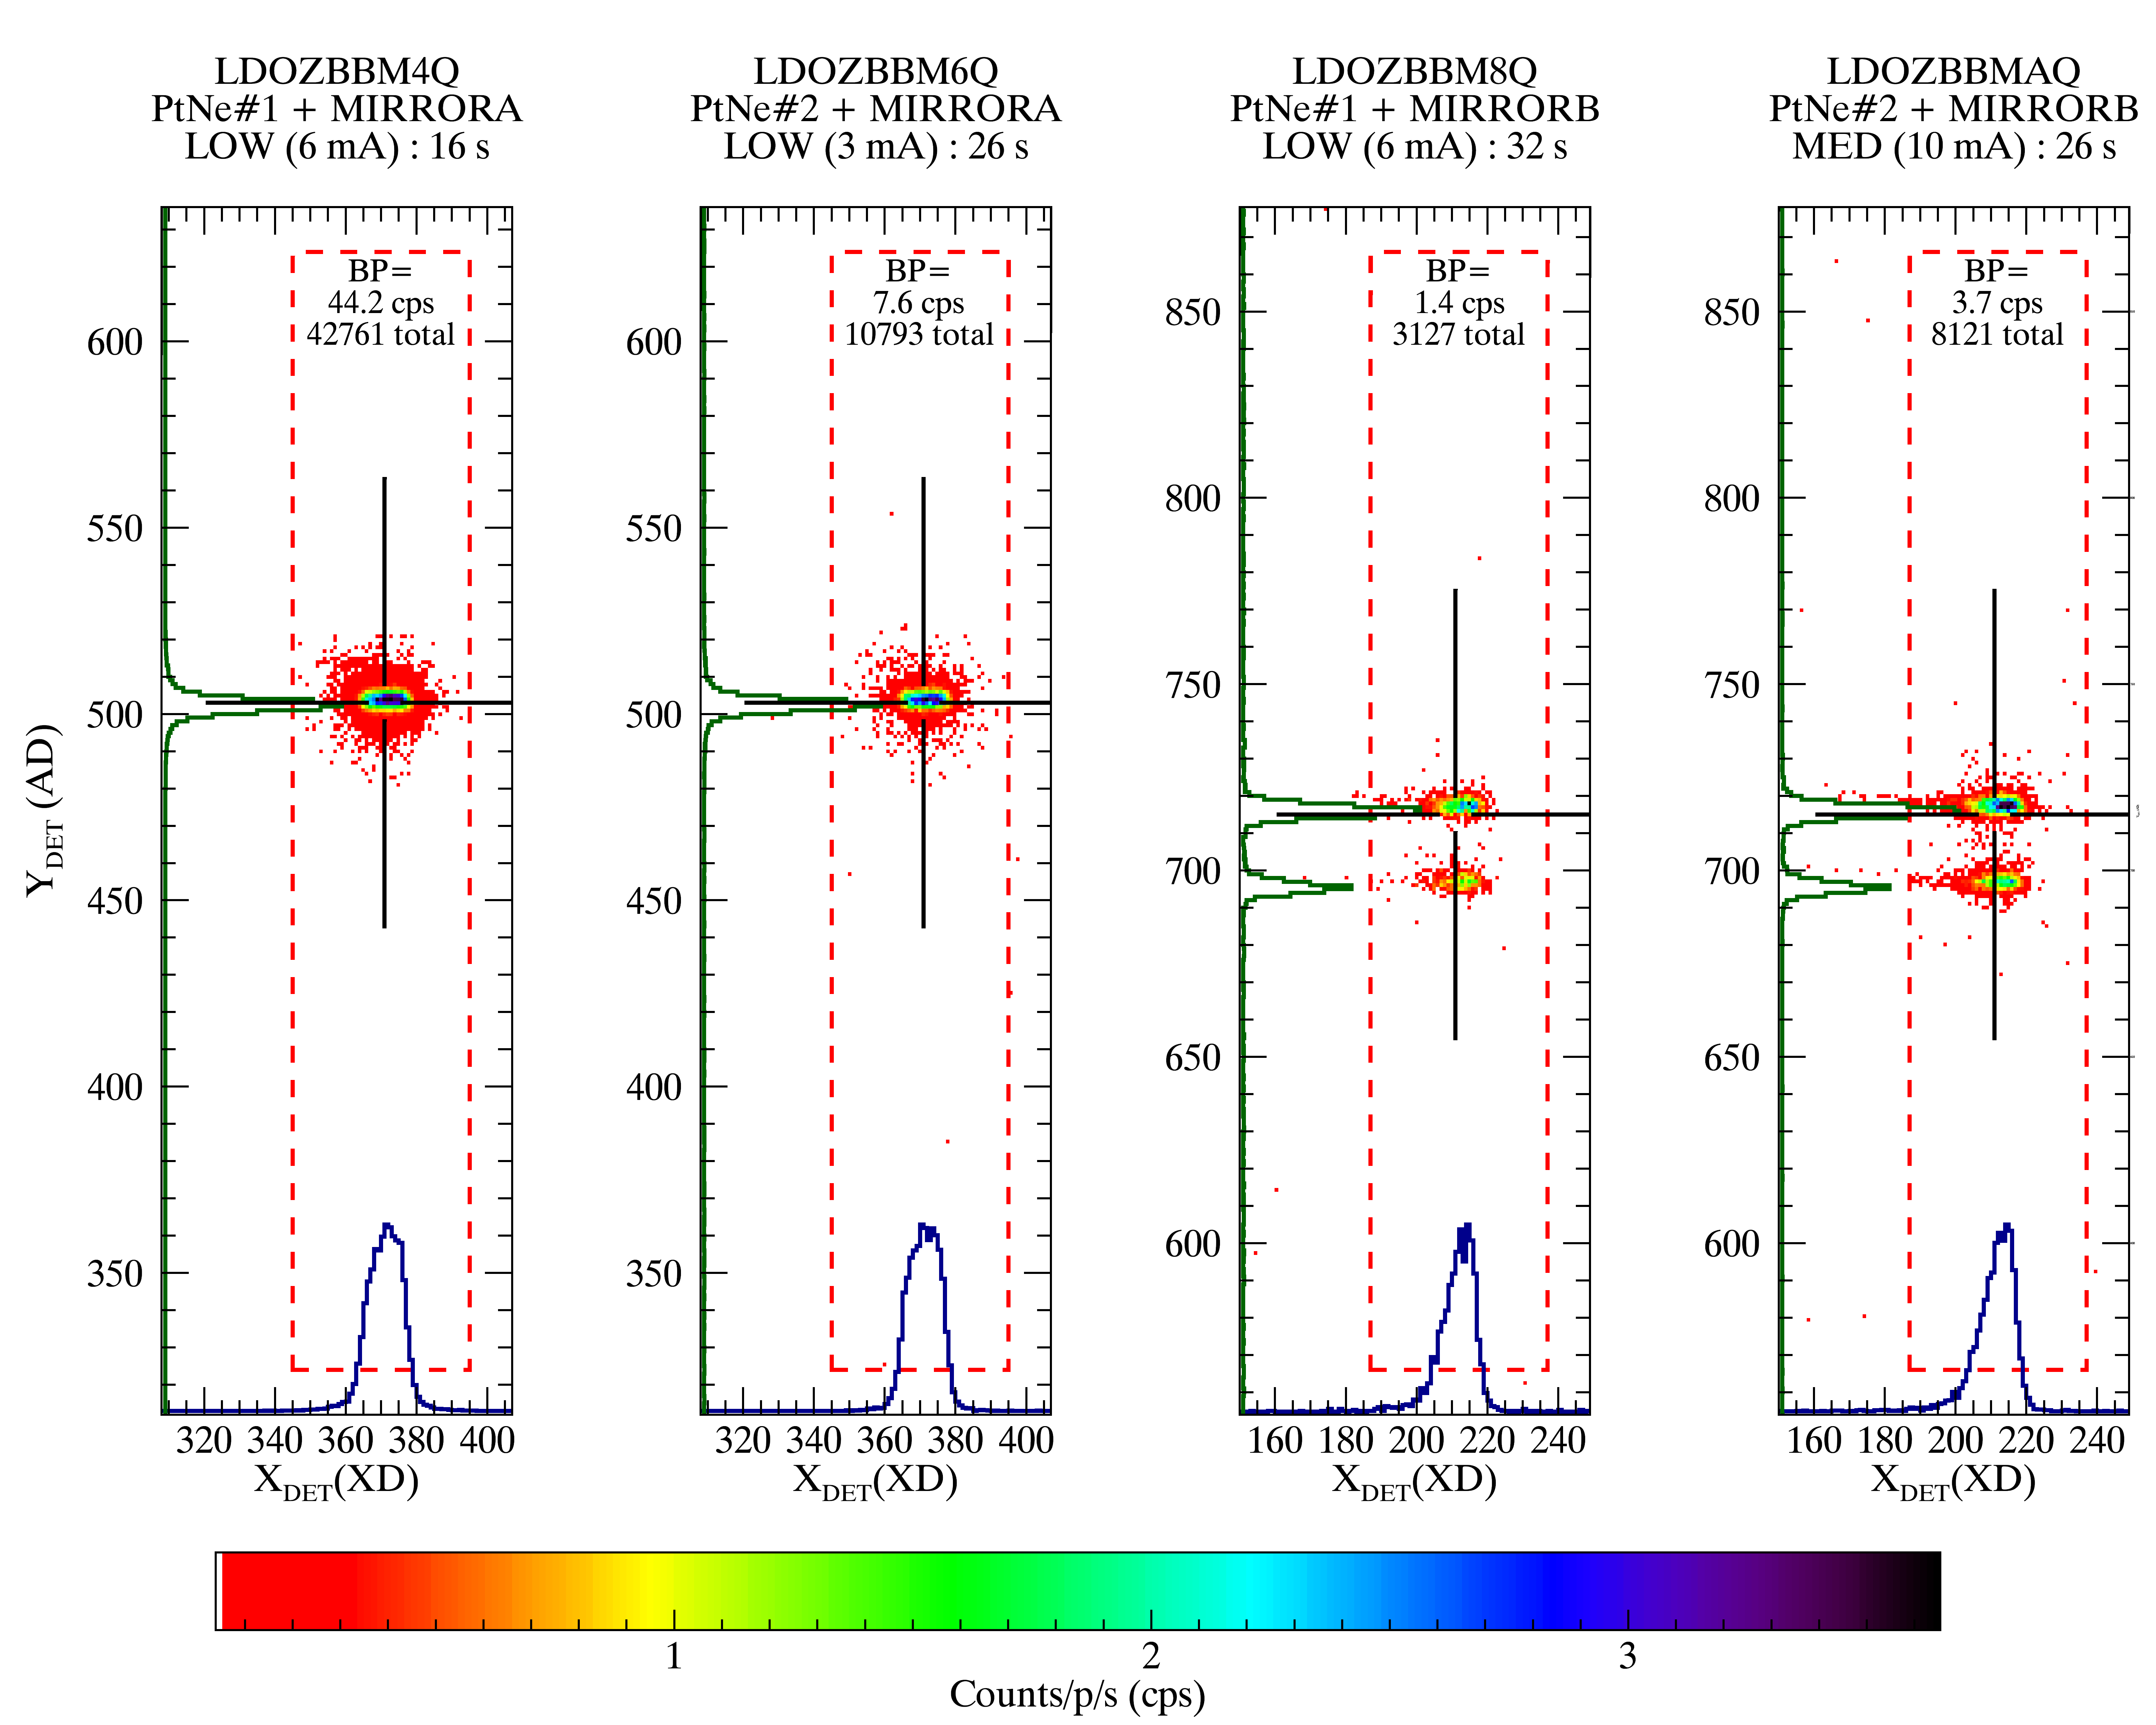
\includegraphics[width=\textwidth]{C24_14857_FP.png}
	\caption{These four panels show a 'family portrait' of the available COS PtNe Lamp + MIRROR combinations possible with ACQ/IMAGE. Panel titles give the lamp and mirror combination, along with the current setting (in milli-amps, mA) and the exposure times in this program.
	These images are in 'detector' coordinates, as used on-board COS.
	The images show the observed counts/pixel/s (cps) as given by the colorbar on the bottom.
	The \textcolor{red}{red} dashed boxes show the Cycle~24 \acqimage~WCA subarrays. At the top of the subarrays, text provides the count rate in the brightest pixel (BP) in units of counts per second per NUV MAMA pixel (cps).
	The \textcolor{blue}{blue} histogram on the bottom edge shows the cross-dispersion (XD) lamp profile in detector 'X' coordinates, while
	the \textcolor{green}{green} histogram on the left edge shows the along-dispersion (AD) lamp profile in detector 'Y' coordinates.
	The cross-hairs show the median location of the given configurations' lamp events within the TA subarray.
	PtNe\#2 lamp was used for all \acqimages~ during Cycle~24, and was operated at LOW current (6~mA) for those using MIRRORA and MEDium current (10~mA) for those using MIRRORB.
	}
	\label{fig:FP}
	\vspace{1.3cm}
	\end{figure}

\end{description}
\vspace{-0.3cm}
\ssection{Conclusions.\label{theend} }
\vspace{-0.3cm}

%%%%%%%%
%Acknowledgements
%%%%%%%%
\vspace{-0.3cm}
\ssectionstar{Acknowledgements}
\vspace{-0.3cm}
%%%%%%%%
%Change History
%%%%%%%%
\vspace{-0.3cm}
%Put instrument, year, and ISR number
\ssectionstar{Change History for COS ISR 2018-XX}\label{sec:History}
\vspace{-0.3cm}
%Put publication date
Version 1: 28-Feb-2018 Original Draft Document
%%%%%%%%
%References
%%%%%%%%
\vspace{-0.3cm}
\ssectionstar{References}\label{sec:References}
\vspace{-0.3cm}

\noindent
Penton, S., 2016, COS Instrument Science Report 2019-09
\\
C22 IHB
C23 IHB
C24 IHB
TAACOS1
TAACOS2
Keyes, T., \& Penton, S. COS 2010-14 (v1) (HST+COS Target Acquisition Guidelines, Recommendations, and Interpretation)\\
Penton, S. 2011, COS TIR 2010-03 (On-Orbit Target Acquisitions with HST+COS)\\
Penton, S. 2016, COS ISR 2016-09 (Cycle~22 HST+COS Target Acquisition Monitoring Summary (HST PID 13972))\\
Penton, S. 2017, COS ISR 2017-18 (Cycle~23 HST+COS Target Acquisition Monitoring Summary (HST PID 14440)\\
Penton, S. \& White, J. 2018, COS ISR 2018-{\bf XX} (HST+COS Target Acquisition Monitoring during Cycles 19-24.)\\

\newpage
%%%%%%%%
%Appendix
%%%%%%%%
\vspace{-0.3cm}
\ssectionstar{Appendix A}\label{sec:Appendix}
\vspace{-0.3cm}
\end{document}
